\chapter{Introduction}
\label{ch:intro}
Autonomous robotics experienced rapid development in the last decades. There are broad ranges of applications from heavy work in the industry to autonomous cars or space exploration. The two latter mentioned applications are very challenging, mainly because they require many abilities that are specific to the area of mobile robotics. Unlike in industry where robots usually perform repetitive tasks in an unchanging environment, the mobile robot must be aware of its surroundings. The robot is usually equipped with various sensors that provide information about the environment to enable the robot to perform complex tasks. Machine perception is a subfield of autonomous robotics which is dedicated to interpreting these sensor's output data.

The thesis is focused mainly on processing the data from a lidar (Light Detection And Ranging) sensor. The lidar is a laser-based rangefinder that uses the passive reflection of a detected object. It has a wide spectrum of usage, and it is also very popular in autonomous robotics. These applications are frequently using a spinning version of the lidar, which can cover $360\degree$ around the robot. In recent years companies like Ouster or Velodyne significantly reduced the cost and improved the quality of this technology, which led to further increasing interest. The classical applications includes collision avoidance \cite{sabatini2007}, SLAM \cite{kohlbrecher2017} or detection \cite{himmelsbach2008}.

The goal of this thesis is to present a detection algorithm for the MBZIRC 2020 (Mohammed Bin Zayed International robotic challenge). The contest aims at the development of autonomous robotics and presents challenging problems that must be resolved before the robots can be applied in the real world. All of the participants are further motivated by the prize money for the winner.

Chapter \ref{ch:intro} presents a problem, used equipment and software. The state-of-the-art methods are also discussed. In Chapter \ref{ch:methods} are proposed general methods that can be used for solving the problem. In Chapter \ref{ch:applications} are introduced tweaks to previously presented methods, which are necessary for our use-case. Chapter \ref{ch:experiment} contains a description of the conducted experiment and performance analysis of all methods. Last Chapter \ref{ch:conclusion} is devoted to the evaluation and conclusion.

\section{State of the art}
Because lidar is the most precise depth measuring sensor, it is often used for object detection in 3D space. Many proposed detectors use various machine learning methods. The SVM method was successfully used for classification before the boom of neural networks \cite{himmelsbach2008}. Nowadays, the most popular solutions are the ones powered by deep neural networks. CNNs (Convolutional Neural Networks), which operate on a 3D voxel map, are often used \cite{zhou2017}. This Voxel network architecture provides an end-to-end solution and can detect and classify on voxel map in one run. Many other architectures, which can improve the performance of such a network, were proposed. For example, slightly different CNN architectures or loss functions \cite{yan2018}. 

These networks have excellent performance, but they are developed mainly for use in autonomous vehicles. That means that they are trained on large annotated datasets, and they are usually computationally intensive (they require GPU). Moreover, the networks are used on quite a dense voxel map, which is generated by lidar with very high vertical resolution. Well known KITTI dataset was captured by lidar with more than four times higher vertical resolution than the lidar used in this thesis \cite{geiger2013}.

Very unpleasant is that the brick is very often hit by only one lidar layer. That is caused by the small size of the brick and low resolution of the lidar. We concluded that using some advanced feature extractor is unnecessarily complex to detect objects which manifest in lidar data as a simple line. Furthermore, these classifiers usually require large annotated datasets that are not available for our problem. Instead, we use more legacy approaches involving mainly line segmentation algorithms.

\section{MBZIRC Contest}
The contest took place in March in Abu Dhabi. The whole competition consisted of three challenges and the grand challenge, which connected all challenges. The first challenge was the only one that was focused solely on UAVs (unmanned aerial vehicles). The goal of the first challenge was to pop multiple big-colored balloons and catch a small ball carried by the organizer's drone. The other two challenges were designed for both UGVs (unmanned ground vehicles) and UAVs. 

The second challenge was about building a wall using robots. Multiple polystyrene bricks were placed in the arena, and the robots should have moved these bricks to the destination area and stack them on top of each other to build the wall. 

The third challenge was to extinguish a fire on the surface of the building model. This task was motivated by the inability of firefighters to extinguish fire inside high-rise buildings in United Arab Emirates. UAVs and UGVs carried tanks full of water and squirted it into the fire dummy. Every team had three rehearsals before the contest, and then two competition attempts for each one of the three challenges. Only the best teams from all three challenges were nominated into the grand challenge, which was limited to just one attempt.

\subsection{Second Challenge}
This thesis is focused on the second challenge, specifically on the ground robot section of the second challenge, so that we provide a more detailed description. Each team is given thirty minutes to explore the arena ($40$m$\times 60$m), localize all interest areas, and build the wall. There are four types of bricks with different colors. All bricks must be very light to enable the UAVs to pick them up. The dimension and colors of the bricks can be seen in Figure \ref{fig:brickdef}. The team obtains points for every placed brick. Bricks with different colors are rewarded by a different number of points. Placing bigger bricks means higher rewards. In addition, the UAV bricks are rewarded by twice as many points as the UGV bricks.

\begin{figure}[H]

\centering
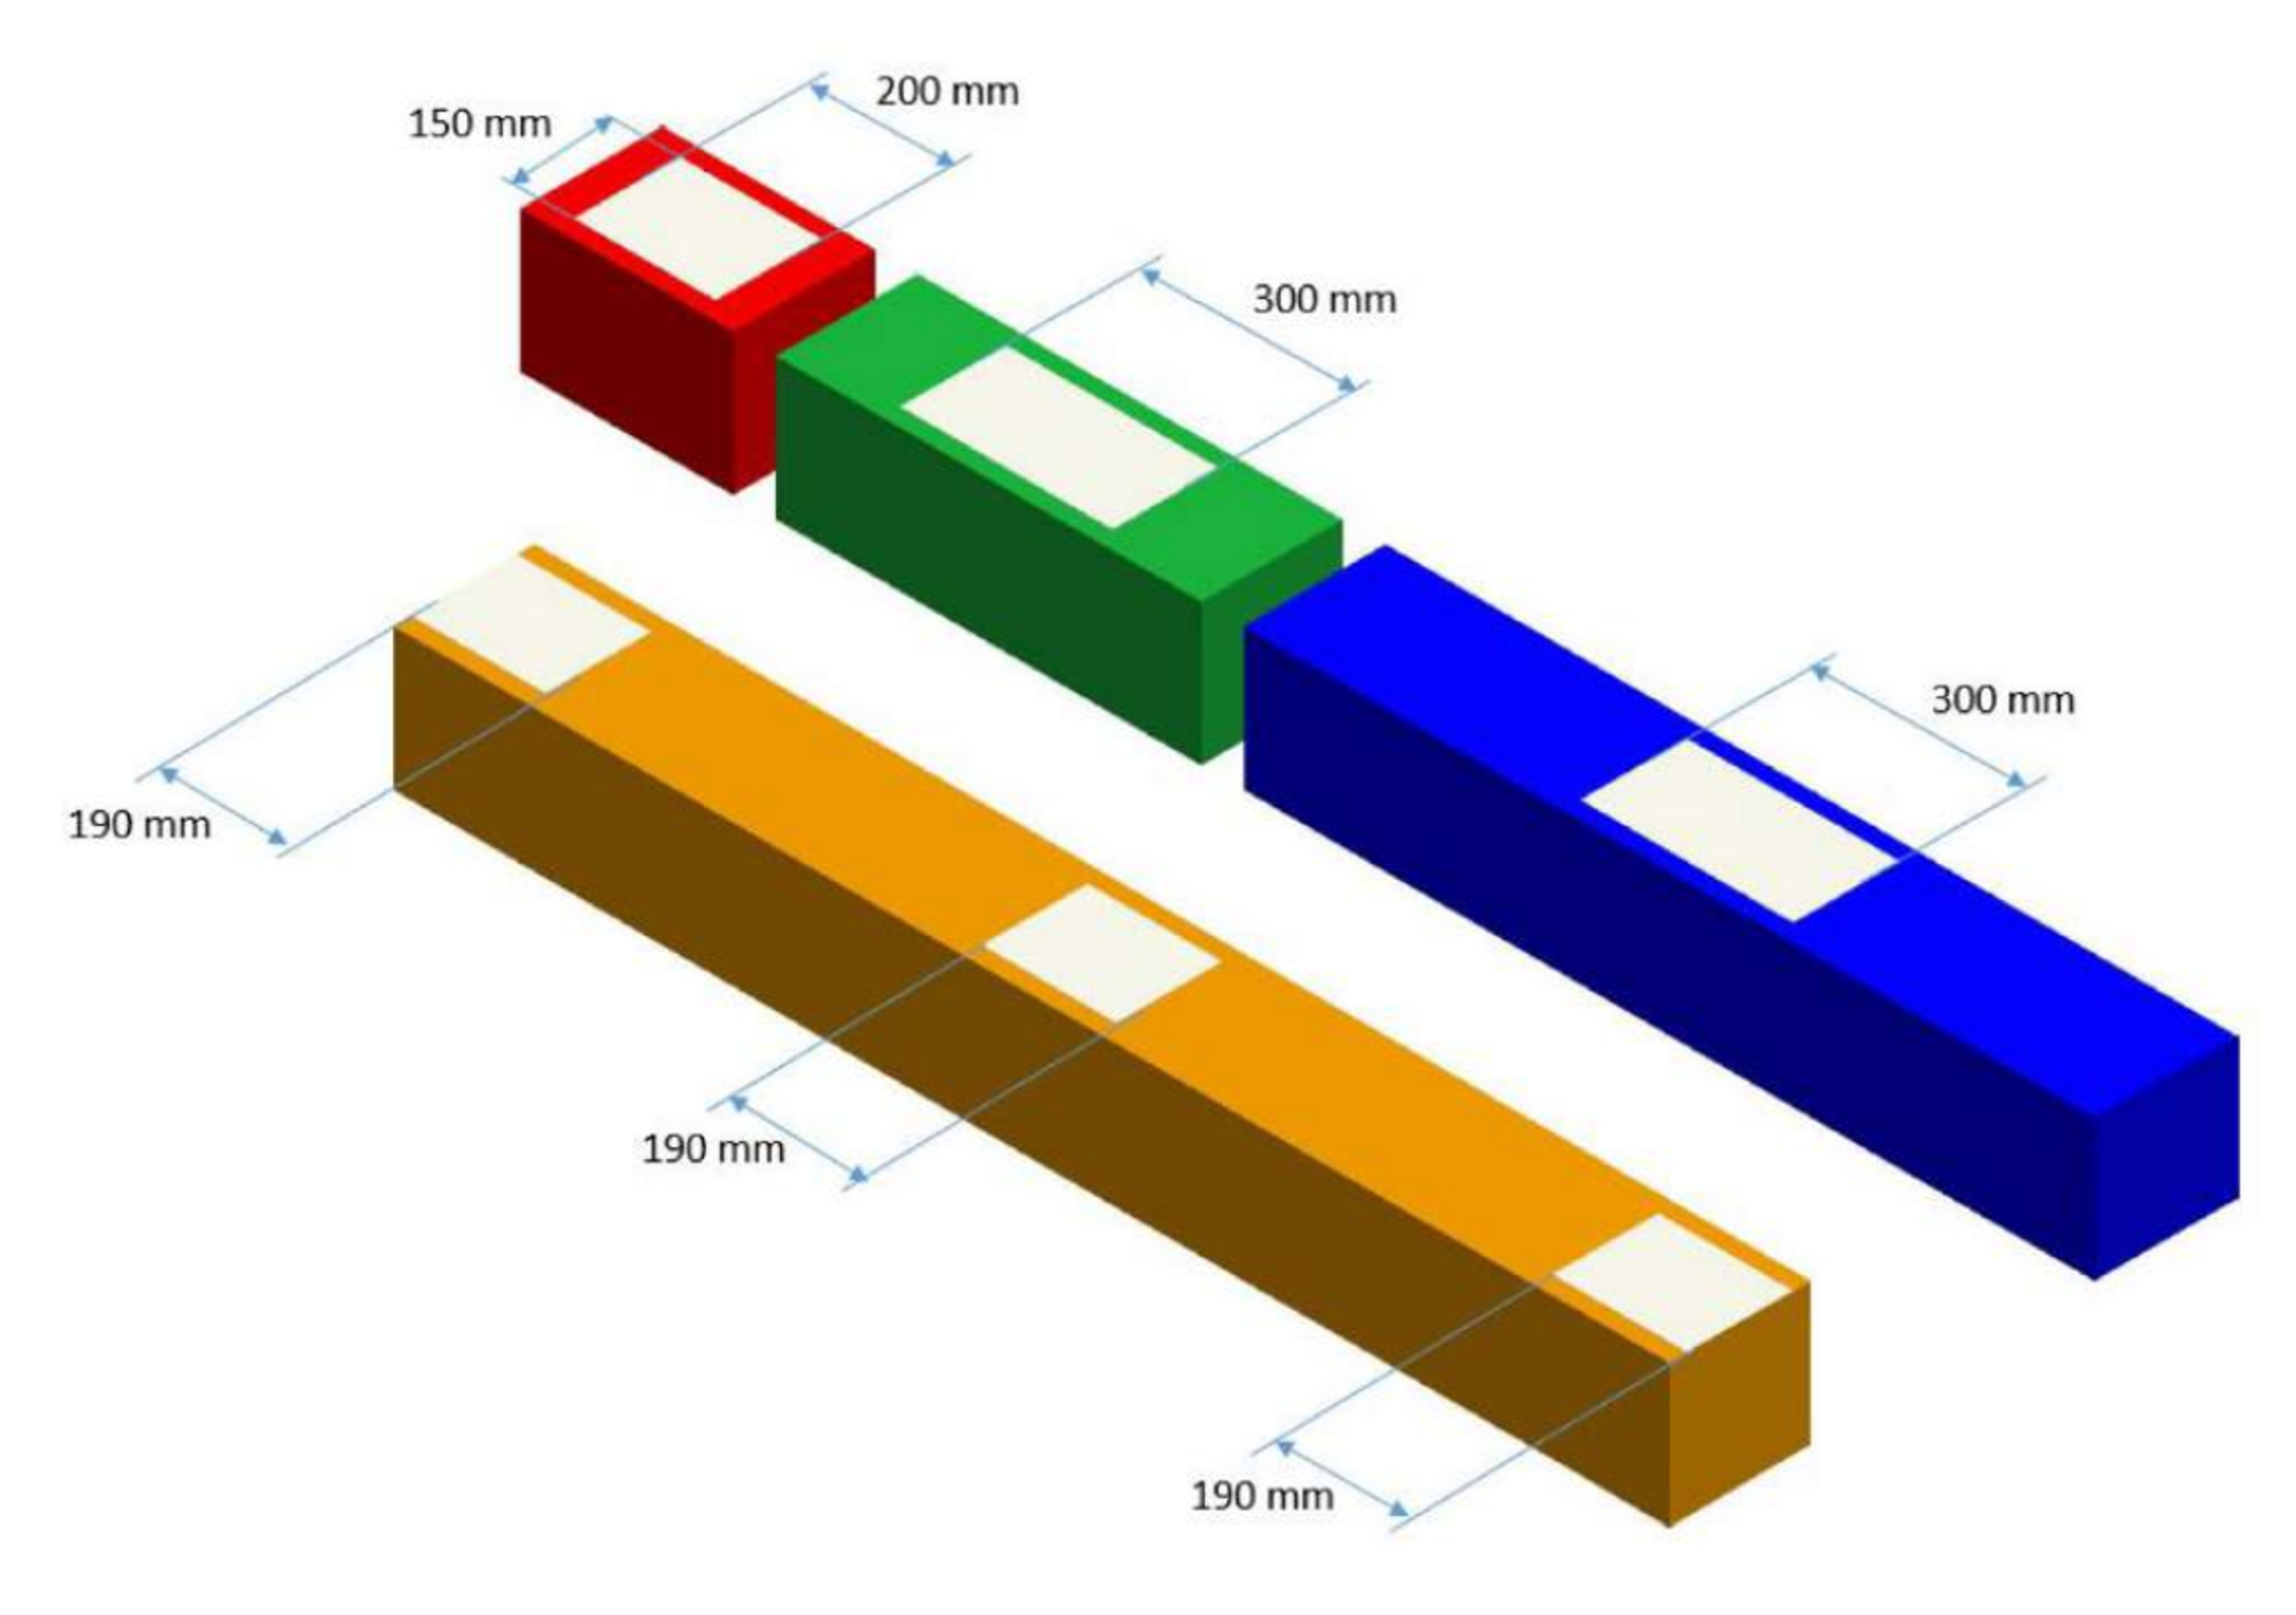
\includegraphics[scale=0.33]{fig/brick_sample.png}
\caption[Bricks definition]{Colors and dimensions of the bricks provided by the organizer.}
\label{fig:brickdef}

\end{figure}

Each brick has a thin metal plate on top of it so that the robots are able to pick them up using electromagnets. At the beginning of the challenge, all bricks are placed in a beforehand unknown position. The initial position of bricks is unknown, but there is a predefined pattern in which the bricks are put together. There are different patterns for the UGV piles of bricks and the UAV piles. The UGV bricks are stacked into the multiple height levels, whereas the UAV bricks are stacked into the width, and all are put on the ground. Due to the low weight of the bricks, it is necessary to put UAV bricks into the rails. Otherwise, the bricks could be easily blown away by the propellers of the drones. Since the UAV bricks are all on the ground level (in the purely horizontal pattern), detecting them with the UAV bottom camera is much easier than using the lidar. That is why we are further concerned only about UGV bricks. These bricks are stacked in the positions displayed in Figure \ref{fig:piledef}.

\begin{figure}[H]

\centering
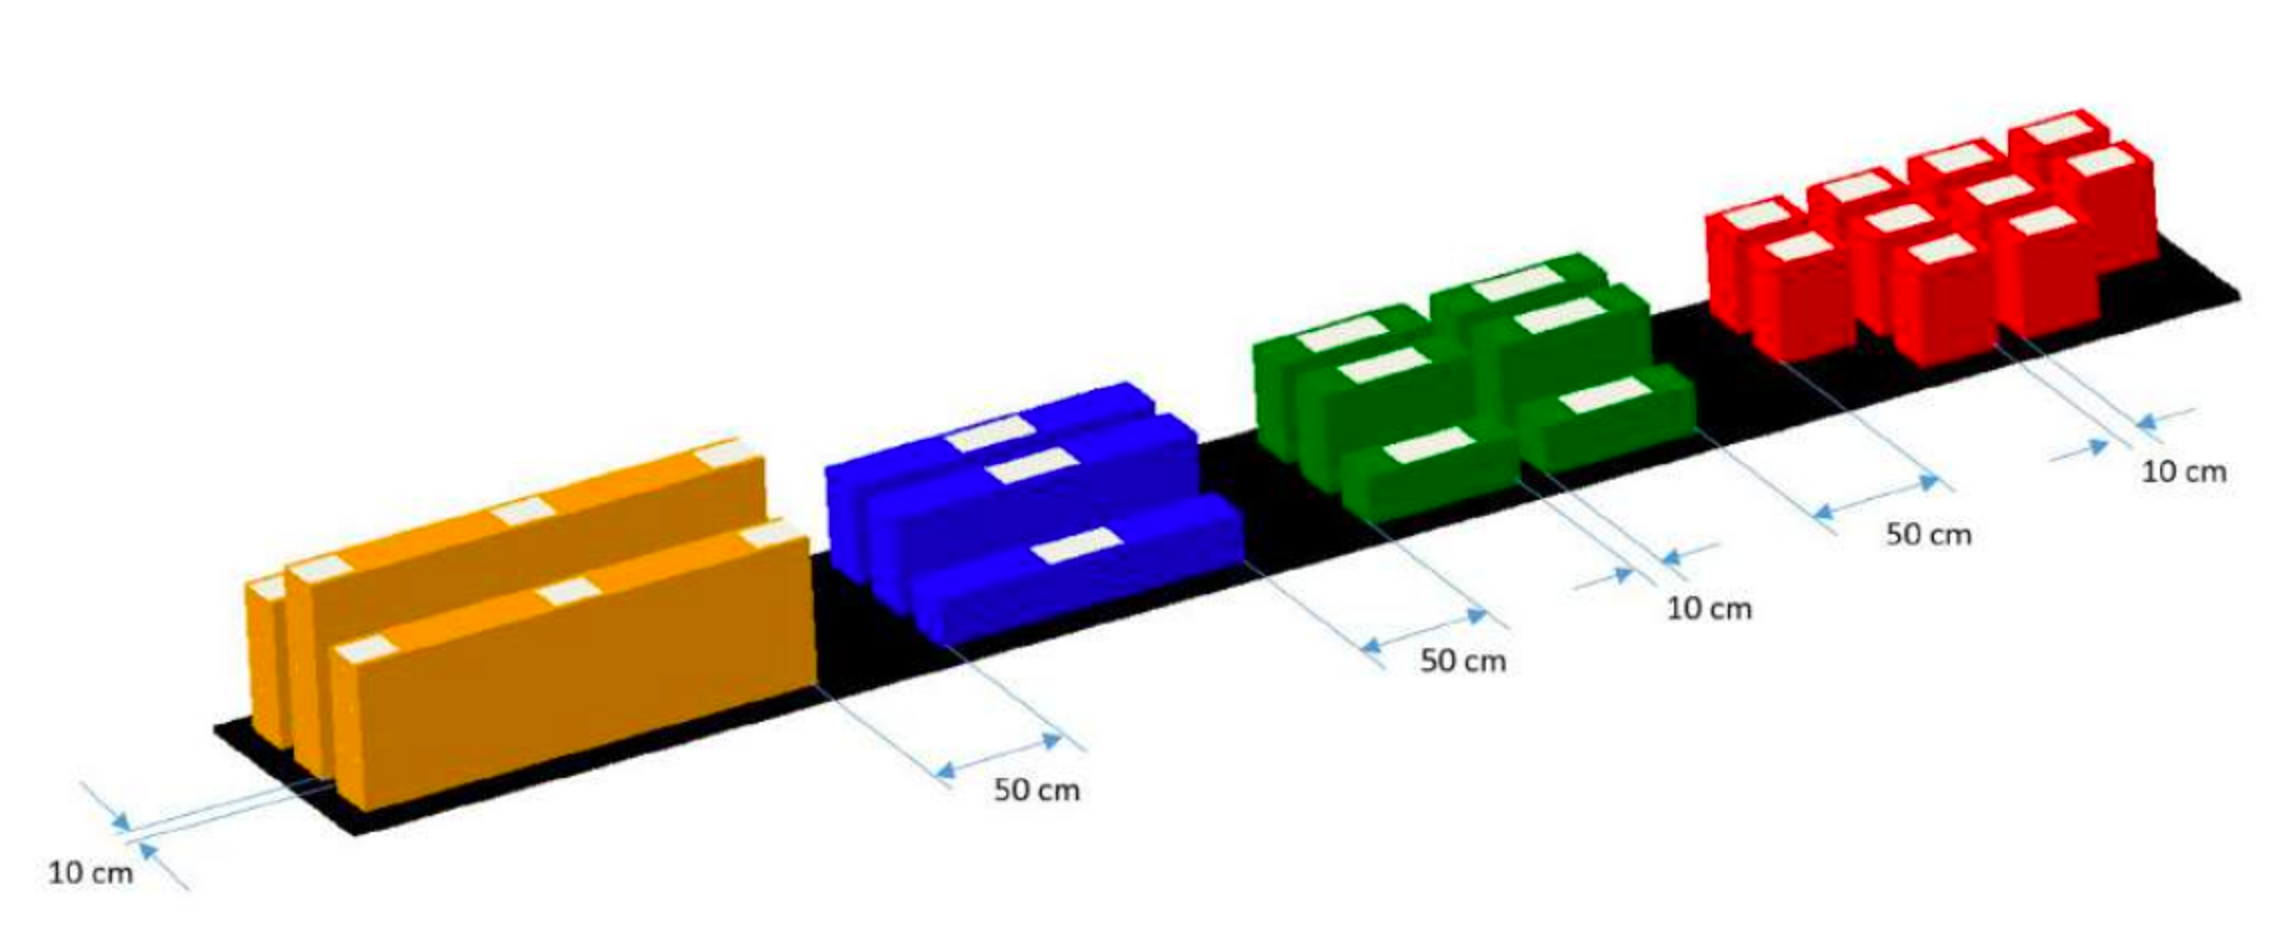
\includegraphics[scale=0.35]{fig/initial_layout.png}
\caption[Initial brick layout]{The positions of the bricks at the beginning of the second challenge.}
\label{fig:piledef}

\end{figure}

Other objects of interest are destinations where the bricks should be placed. The robots must look for them during the exploration. UGV brick's destination is marked by a checker pattern. Detecting the pattern was very challenging because the exact shape was not known until the second rehearsal. The final form of the pattern is shown in Figure \ref{fig:checker}. Although we are not concerned about the UAV bricks, the destination of the UAV bricks is a vertical object, so it is much easier to detect it from the ground using the lidar. The UAV bricks destination is a wall, as seen in Figure \ref{fig:uavdest}. Bricks should be placed on top of this wall. The metal plate on top of each brick shifts the center of mass to the top and make the brick very susceptible to rolling. That is why are the auxiliary handles mounted on the top of the UAV destination wall. At the beginning of the challenge, each team is given the instructions which describe how the wall should look like at the end. When the built wall does not fit the instructions, the team gets a penalty and gains fewer points for inaccurately placed bricks.


\begin{figure}[H]
\centering
\begin{subfigure}{.3\textwidth}
  \centering
\vspace{18mm}
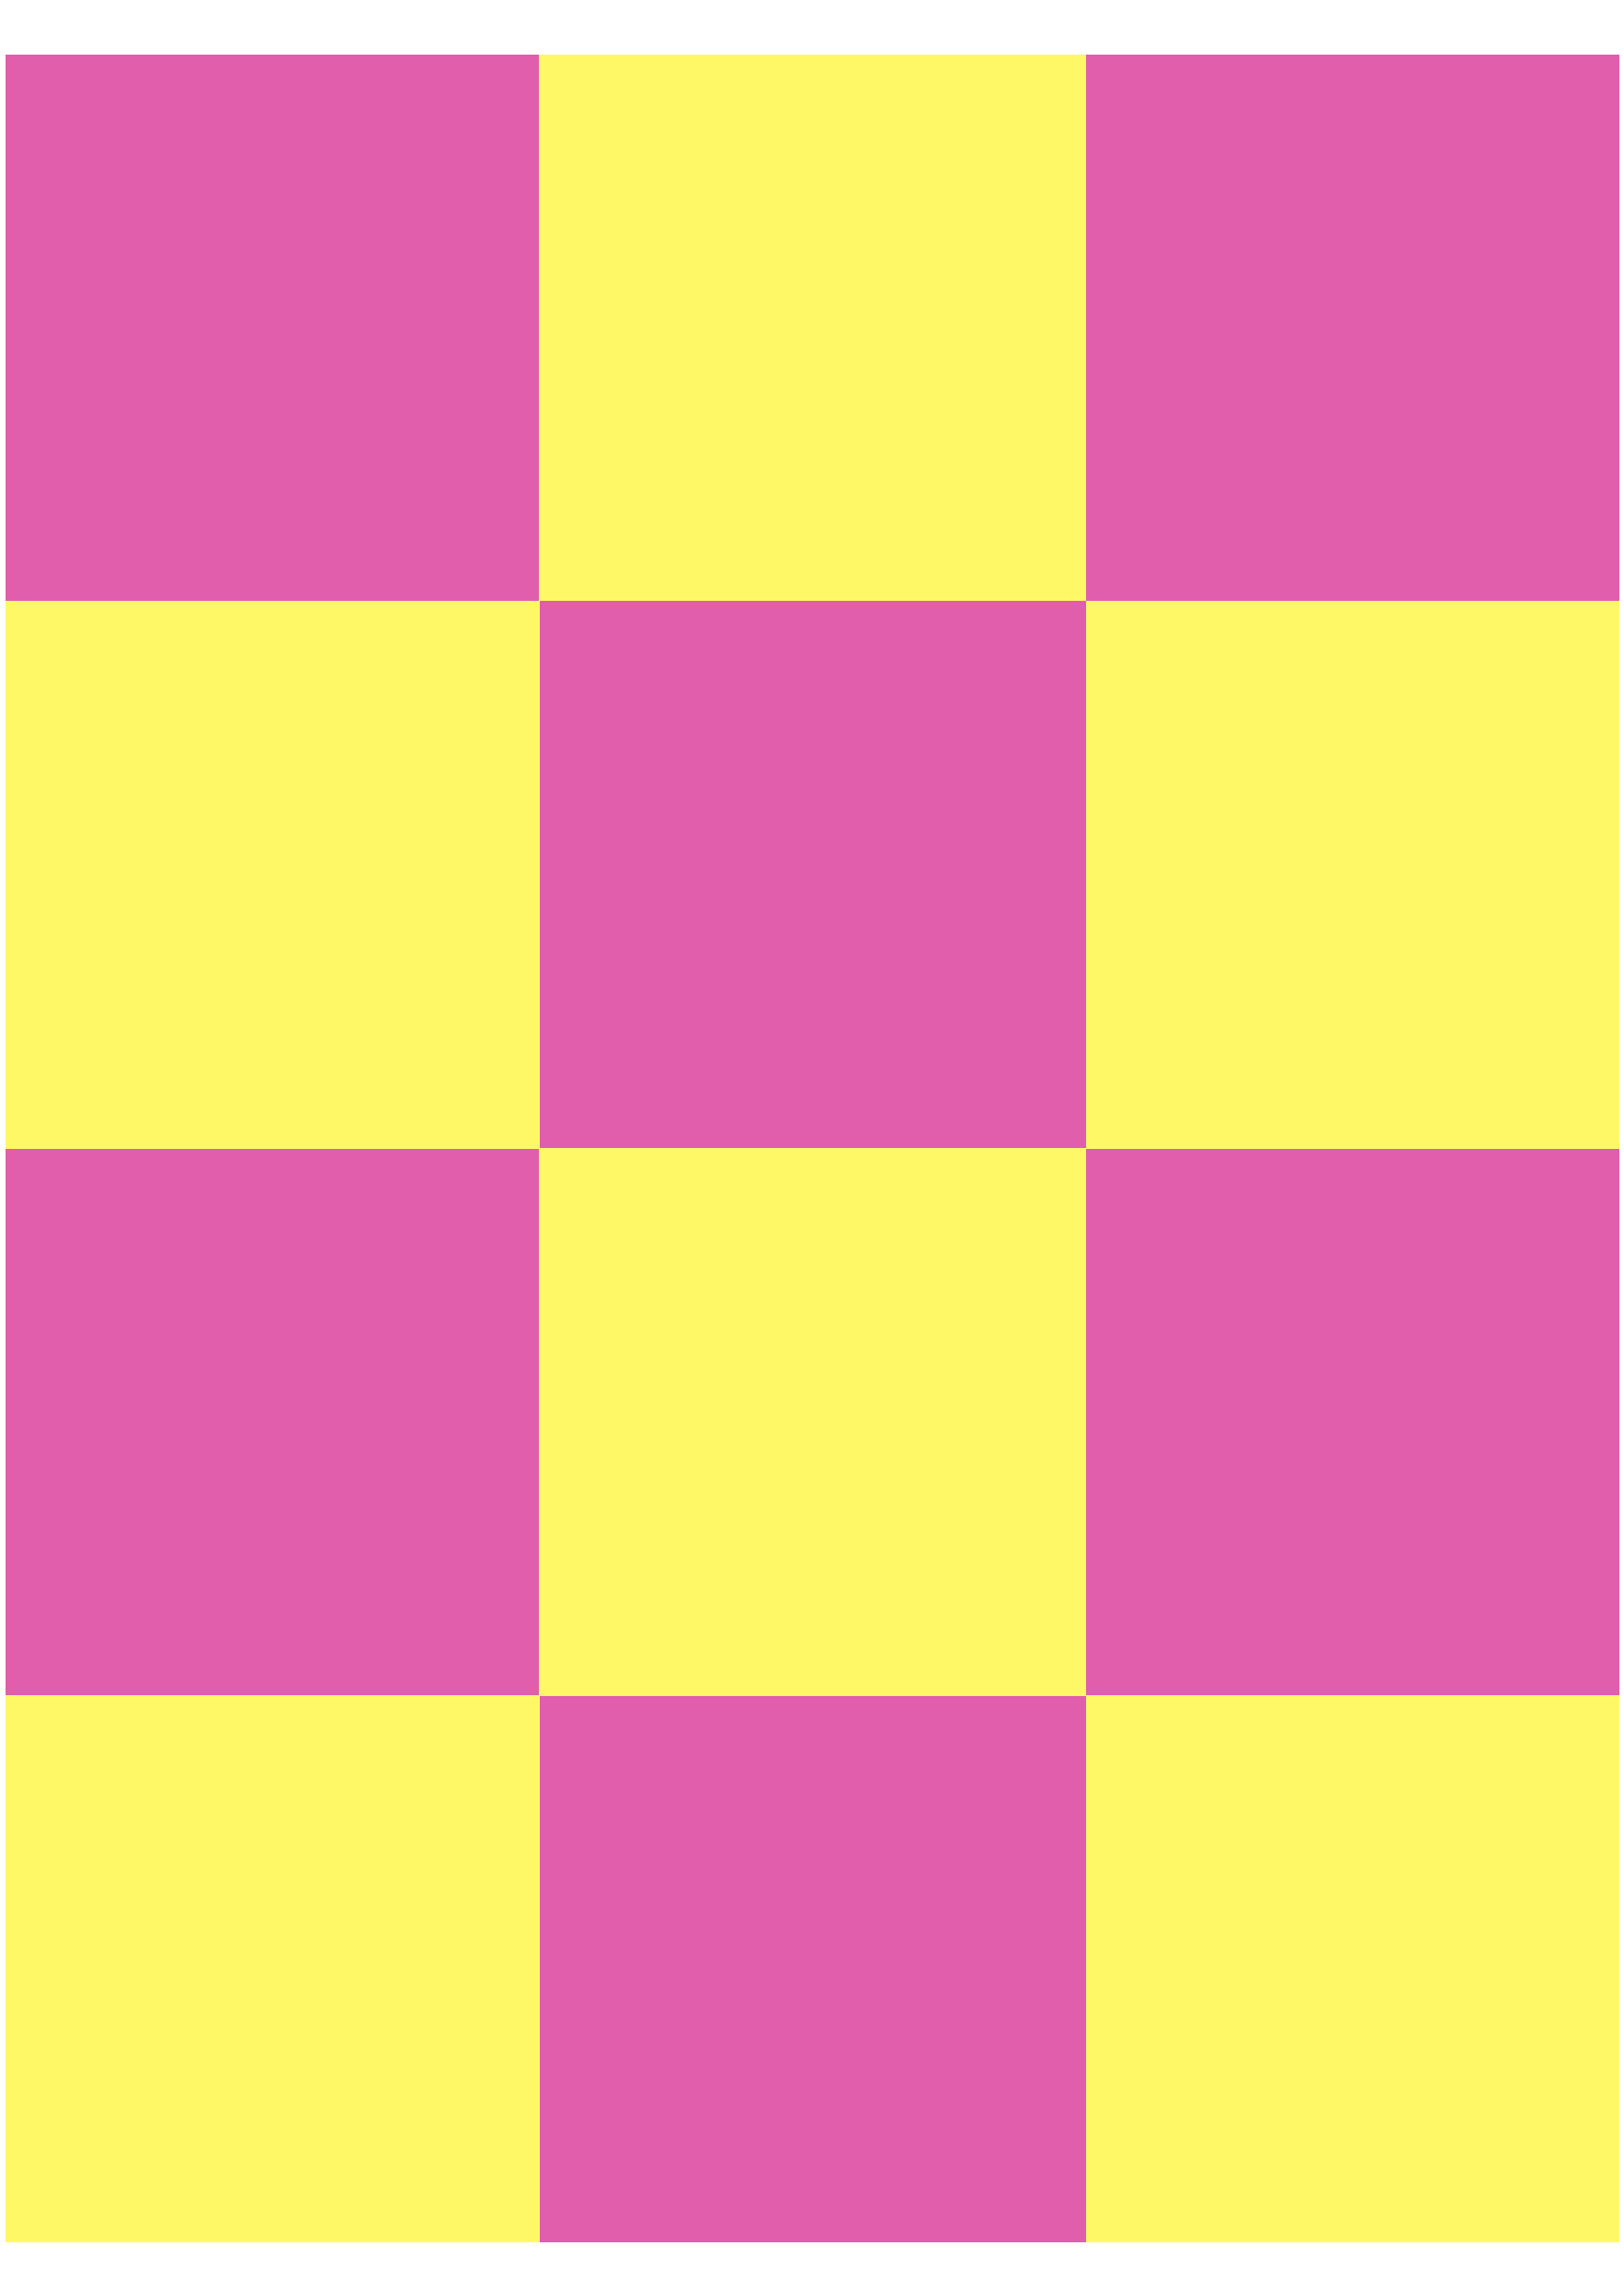
\includegraphics[scale=0.1]{fig/pattern.pdf}
\vspace{18mm}
\caption[UGV destination]{UGV destination pattern.}
\label{fig:checker}
\end{subfigure}
\begin{subfigure}{.65\textwidth}
  \centering
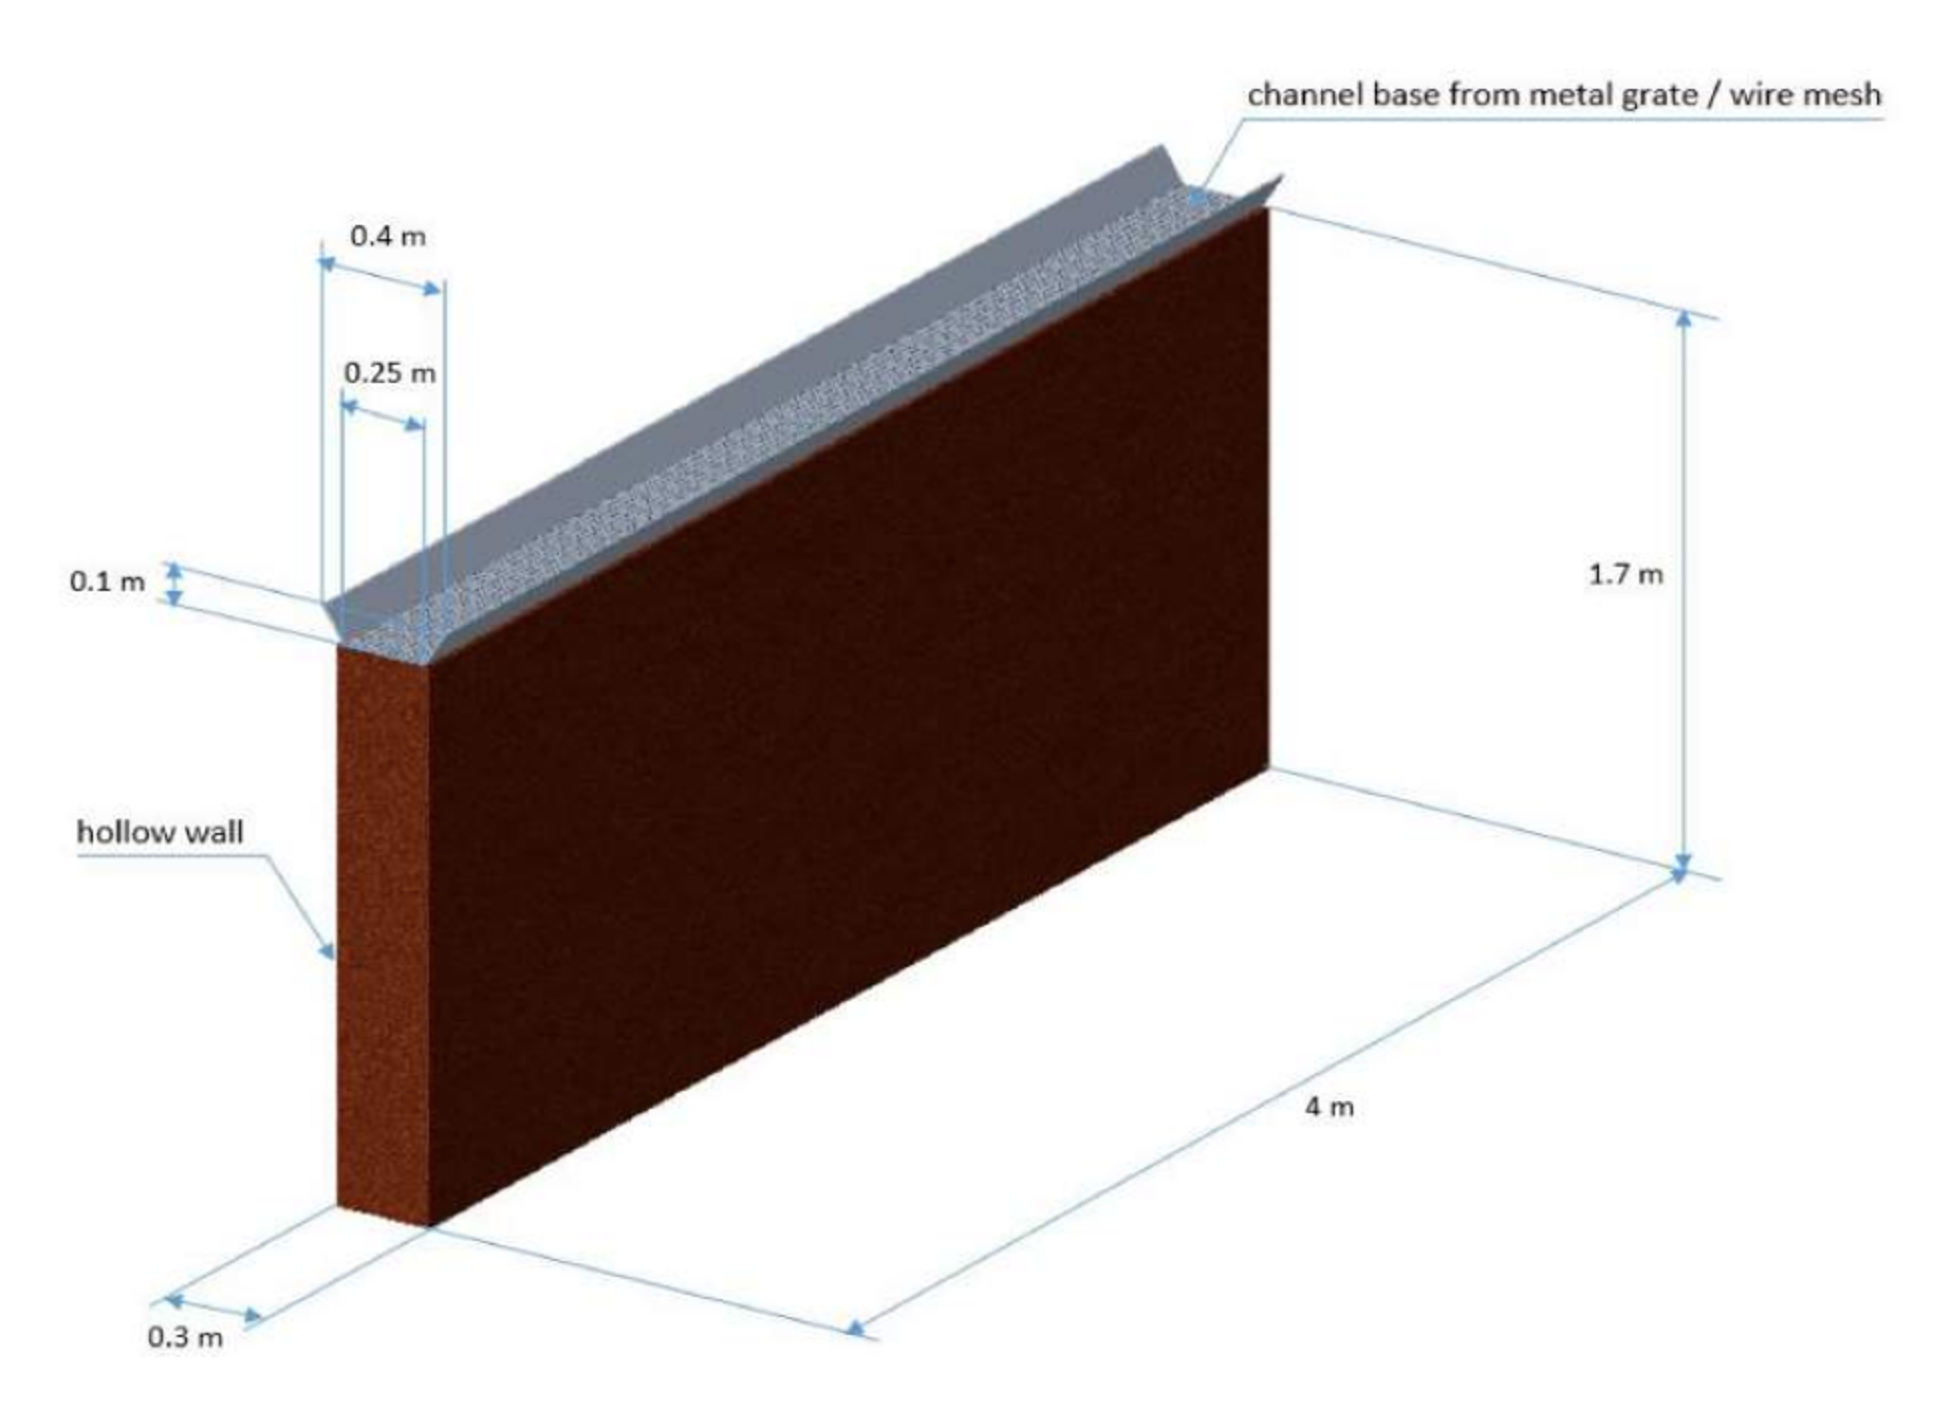
\includegraphics[scale=0.35]{fig/wall_sample.png}
\caption[UAV destination]{UAV destination}
\label{fig:uavdest}
\end{subfigure}

\caption[Brick destinations]{Description of target places for UAVs and UGVs. Each square in the UGV pattern has a width of $0.1$m. The pattern consists of two $4\times0.4$m segments, which are connected into the \textit{L} shape. Whole UAV destination consists of four similar segments arranged into the \textit{W} shape with right angles.}
\label{fig:dest}
\end{figure}


\section{Equipment}
For the sake of completeness, it is necessary to describe what exact equipment was available. We used \textbf{Clearpath Husky A200}, which is a wheeled robot designed for outside robotics. The robot was equipped with many additional devices. \textbf{Intel NUC} was used as a computer to run the code and control the robot. The \textbf{Kinova robotic arm} was mounted on top of the Husky robot to manipulate the bricks. Two \textbf{12V electromagnets} were attached to the end-effector to enable the arm to grip the bricks. It would be tough to grip the bricks without any feedback loop to the hand. For visual servoing and proper gripping, we placed \textbf{Intel Realsense} camera close to the end of the arm. It is also possible to obtain feedback from electromagnets thanks to hall effect sensors and decide whether the brick is gripped correctly. For the localization, collision avoidance and detection was used \textbf{Velodyne VLP-16} lidar sensor. Lastly, to move the bricks around the arena, we created a handmade cargo area that can contain up to six bricks and attached it to the rear bumper. It was not possible to carry more bricks mainly because of restrictions on the robot's size and also due to the limited range of Kinova arm. The whole setup is captured in Figure \ref{fig:husky}.

\begin{figure}[H]
\centering
\includegraphics[scale=0.275]{fig/husky.png}
\caption[UGV setup]{Clearpath Husky A200 adjusted for the second challenge.}
\label{fig:husky}

\end{figure}

\subsection{Velodyne VLP-16}
This thesis deals mainly with lidar data. Therefore, the following subsection provides a more detailed description of the lidar sensor. Inside the VLP-16 puck, there is a rotating infrared laser of class one, which measures the distance using the time of flight principle. A 12V power supply powers lidar and the data are transferred via UDP packets over the ethernet. The configuration of the Velodyne lidar used for the contest is described in Table \ref{tab:lidar}. The lidar can be set up with a slightly better resolution, but there is a trade-off between resolution and frequency, and we preferred higher frequency over the resolution.

\begin{table}[H]
\centering
\caption{Parameters of the VLP-16 lidar sensor.}
\begin{tabular}{lr}
\toprule
Parameter & Value \\
\midrule
Layers [-]                            & 16   \\ 
Maximal Range [m]                         & 100  \\
Vertical FOV [$\degree$]          & $\pm15$   \\ 
Vertical resolution [$\degree$]   & 2    \\ 
Horizontal FOV [$\degree$]        & 360  \\ 
Horizontal resolution [$\degree$] & 0.4  \\ 
Frequency [Hz]                    & 20    \\ 
Precision [m]                     & $\pm0.03$ \\ 
\bottomrule
\end{tabular}
\label{tab:lidar}
\end{table}

\section{Software}
The operating system which is installed on the Intel NUC hard drive is Ubuntu 18.04. All necessary subroutines for controlling the robot are run by the Robot Operating System (ROS) \cite{ros}. That is a flexible framework for operating various robots or multi-robot systems. It offers many different tools and packages which can vastly simplify development, debugging, and deploying of any robotic platform. ROS is written in C++, but offers bindings to other modern languages such as Python or Ruby. Our work is implemented in C++ because it achieves the best performance in terms of execution time, and it has the best community support. ROS precisely defines how the files must be structured within the package. ROS also offers a high encapsulation level where each executable is run as a node that can communicate with other nodes using the predefined protocols. The protocols are defined in the form of ROS messages, which are used in two different ways. One possibility is to transmit the data via the ROS topics. Topics represent the classical producer-consumer scheme, where multiple listeners can be joined to a single topic, whereas the publisher doesn't receive anything. The other possibility is a so-called service server that returns something on each request. The most important node is the ROS core, which runs the ROS master and the parameter server. ROS also provides advanced logging and package \textit{rosbag}, which can record any specified topic and save it for replay.

It is vital to know the precise location of the robot inside the arena. For localization, the robot uses a probabilistic Monte Carlo method, which is sometimes called the particle filtering. This algorithm fuses data from range finder and odometry and creates multiple hypotheses (particles) of the robot's position and rotation. Each hypothesis’s quality is evaluated by approximating posterior probability within a standard Bayesian formulation of the localization problem \cite{dellaert1999, thrun2000}. Firstly, it is necessary to create a map when the robot is placed in a new environment. There is a ROS package called Gmapping, which can simultaneously create the map and navigate the robot using the particle filter. When the map is created, it is not further necessary to run the Gmapping node because only the localization is needed. For the Monte Carlo localization on a predefined map, the ROS package called AMCL is used.
